\documentclass[journal]{IEEEtran}
\usepackage[english]{babel}

\usepackage{amssymb, amsmath} %Paquetes matemáticos de la American Mathematical 
\usepackage[utf8]{inputenc}
\usepackage{graphicx}
\usepackage{float}
\usepackage{hyperref}
\usepackage{listings}
\usepackage{xcolor}

\definecolor{codegreen}{rgb}{0,0.6,0}
\definecolor{codegray}{rgb}{0.5,0.5,0.5}
\definecolor{codepurple}{rgb}{0.58,0,0.82}
\definecolor{backcolour}{rgb}{0.95,0.95,0.92}
% Definicio de estilo para el codigo fuente que se cita
\lstdefinestyle{mystyle}{
    backgroundcolor=\color{backcolour},   
    commentstyle=\color{codegreen},
    keywordstyle=\color{magenta},
    numberstyle=\tiny\color{codegray},
    stringstyle=\color{codepurple},
    basicstyle=\ttfamily\footnotesize,
    breakatwhitespace=false,         
    breaklines=true,                 
    captionpos=b,                    
    keepspaces=true,
    numbers=left,                    
    numbersep=5pt,                  
    showspaces=false,                
    showstringspaces=false,
    showtabs=false,                  
    tabsize=2,
}
\lstset{style=mystyle}

\renewcommand{\lstlistingname}{Código}

\ifCLASSINFOpdf

\else

\fi
\begin{document}

\title{Ejercicio 3 - tema 7 \\ Administración de data files}
%
\author{Vicente Romero Andrade}

\markboth{Ejercicio 3 - tema 7 Administración de data files, Julio~2021}%
{Shell \MakeLowercase{\textit{et al.}}: }
% The only time the second header will appear is for the odd numbered pages

\maketitle


\IEEEpeerreviewmaketitle

\section{Objetivo}
% The very first letter is a 2 line initial drop letter followed

\IEEEPARstart{E}{l} objetivo es Poner en práctica las tareas de administración básicas 
que se asocian con el mantenimiento de data files: cambiar su ubicación, poner un data 
file fuera de línea, etc.

\section{Desarrollo}
\subsection{sentencias}
\begin{lstlisting}[language=sql, caption=s-00-datafiles.sql,label={lst:codigo1}]
  whenever sqlerror exit rollback
  set serveroutput on
  connect sys/system2 as sysdba
  --A
  alter database datafile '/u01/app/oracle/oradata/VRABDA2/store_tbs_multiple_01.dbf' offline;
  alter database datafile '/u01/app/oracle/oradata/VRABDA2/store_tbs_multiple_02.dbf' offline;
  alter database datafile '/u01/app/oracle/oradata/VRABDA2/store_tbs_multiple_03.dbf' offline;
  --B
  alter tablespace store_tbs_multiple offline normal;
  --C
  connect VRA_TBS_MULTIPLE/VRA_TBS_MULTIPLE
  SELECT count(*) FROM VRA_TBS_MULTIPLE;
  --D
  connect sys/system2 as sysdba
  SELECT
    FILE_NAME,
    FILE_ID,
    STATUS
  FROM DBA_DATA_FILES WHERE TABLESPACE_NAME ='STORE_TBS_MULTIPLE';
  --E
  alter tablespace STORE_TBS_MULTIPLE 
  rename
    '/u01/app/oracle/oradata/VRABDA2/store_tbs_multiple_01.dbf',
    '/u02/app/oracle/oradata/VRABDA2/store_tbs_multiple_02.dbf',
    '/u03/app/oracle/oradata/VRABDA2/store_tbs_multiple_03.dbf'
  to 
    '/u03/app/oracle/oradata/VRABDA2/store_tbs_multiple_013.dbf',
    '/u02/app/oracle/oradata/VRABDA2/store_tbs_multiple_023.dbf',
    '/u01/app/oracle/oradata/VRABDA2/store_tbs_multiple_031.dbf';
  alter tablespace store_tbs_multiple online;
  --F
  alter database move
  datafile '/u03/app/oracle/oradata/VRABDA2/store_tbs_multiple_013.dbf'
  to '/u01/app/oracle/oradata/VRABDA2/store_tbs_multiple_01.dbf' reuse;
  alter database move
  datafile '/u02/app/oracle/oradata/VRABDA2/store_tbs_multiple_023.dbf'
  to '/u02/app/oracle/oradata/VRABDA2/store_tbs_multiple_02.dbf' reuse;
  alter database move
  datafile '/u01/app/oracle/oradata/VRABDA2/store_tbs_multiple_031.dbf'
  to '/u03/app/oracle/oradata/VRABDA2/store_tbs_multiple_03.dbf' reuse;
  --G
  !mv /u01/app/oracle/oradata/VRABDA2/store_tbs01.dbf /u01/app/oracle/oradata/VRABDA2/store_tbs01.dbfcopy
  -- Solo falla si se usa algo de ese datafile -1
  -- No se puede 2
  -- Se pone offline de manera exitosa
  -- Si se detiene la instancia
  -- Si se inicia sin problemas
  -- pasos para recuperar
  SHUTDOWN IMMEDIATE;
  STARTUP MOUNT;
  alter database datafile '/u01/app/oracle/oradata/VRABDA2/store_tbs01.dbf' offline for drop;
  ALTER DATABASE OPEN; -- A partir de aqui recuperar con archivos SQL
  whenever sqlerror continue  
\end{lstlisting}

\begin{figure}[H]
  \centering
  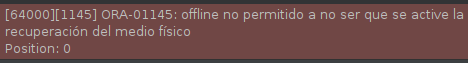
\includegraphics[scale=.35]{captura_a.png}
   \caption{Salida punto A}
   \label{fig:validador_1}
\end{figure}
\subsubsection{¿Qué sucede intentar poner al data file store\_tbs\_multiple\_01.dbf en modo offline?}
No se permite poner el datafile en offline.
\begin{figure}[H]
  \centering
  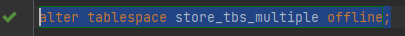
\includegraphics[scale=.35]{captura_b.png}
   \caption{Salida punto B}
   \label{fig:validador_2}
\end{figure}
\subsection{¿Cuál será la forma correcta de proceder?}
Poniendo offline todo el tablespace
\begin{figure}[H]
  \centering
  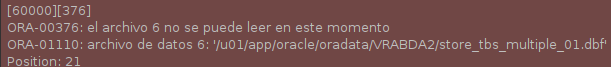
\includegraphics[scale=.35]{captura_c.png}
   \caption{Salida punto C}
   \label{fig:validador_3}
\end{figure}
\subsection{¿Qué sucede si el usuario creado anterior intenta hacer un conteo de los registros de la tabla long\_strings?}
En este caso se uso la tabla str y no se permite la consulta ya que esta offline el tablespace
\begin{figure}[H]
  \centering
  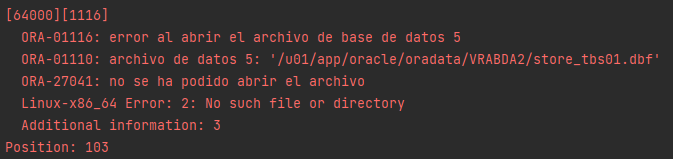
\includegraphics[scale=.35]{captura_g-1.png}
   \caption{Salida punto G}
   \label{fig:validador_4}
\end{figure}
\subsubsection{¿Qué le pasa a la instancia una vez que se ha eliminado el data file?}
No ocurre nada, pero al hacer una consulta a alguna tabla de ese tablespace esta fallara
\begin{figure}[H]
  \centering
  
\includegraphics[scale=.35]{captura_g-2.png}
   \caption{Salida punto G offline tablespace}
   \label{fig:validador_5}
\end{figure}
\subsubsection{Suponer que el DBA se percata del problema y decide poner offline al otro data file que integra al TS. ¿Qué sucederá?}
Esto fallara ya que se tiene que activar la reculeración del datafile dañado o perdido.
\subsubsection{Suponer que el DBA intenta marcar al tablespace en modo offiline, ¿Qué sucederá?}
Si se pone offline de manera satisfactoria.
\subsubsection{¿Qué sucede si el DBA intenta detener la instancia?}
Se detiene correctamente
\subsubsection{¿Qué sucede si el DBA intenta iniciar la instancia con el data file perdido?}
Fallará ya que primero se tiene que recuperar el datafile perdido
\subsubsection{El DBA se percata que no se cuenta con respaldo físico del data file. Sin embargo cuenta con scripts SQL para recuperar los datos. Aplicar las
sentencias SQL necesarias para que el tablespace vuelva a estar en modo online y poder así iniciar la ejecución de las sentencias SQL.}
Primero se aplica drop al datafile, se inicia la instancia y se corren las sentencias sql de respaldo.
En algunos casos seria recomentable crear otro datafile para conservar el espacio original.
\section{Conclusiones}
En este ejercicio se revisó la administración de los datafiles, estos tienen sus dificultades ya 
que hay que tener presentes cuales pertenecen a un determinado tablespace.
\ifCLASSOPTIONcaptionsoff
  \newpage

\fi

\end{document}
